\urldef\urlbtcbook\url{https://github.com/bitcoinbook/bitcoinbook/blob/develop/ch06.asciidoc}

In this section, we will discuss the basics of the Bitcoin transaction protocol.
We will find definitions that we will use later in~\cref{sec:atom:atomic-swap} to construct an atomic swap protocol.
The primary reference of this section is the book Mastering Bitcoin by Andreas Antonopoulos~\cite{antonopoulos2014mastering}.

\subsection{Bitcoin Transaction Protocol}\label{subsec:pre:bitcointx}

A \emph{Bitcoin Transaction} is a data structure that allows transferring value between participants of the network.
In Bitcoin, there are no user balances or user accounts.
Instead, the UTXO model (unspent transaction outputs) is employed.
A UTXO is an output constructed in a previous transaction that holds value in the form of an amount expressed in
Bitcoin (more precisely in Satoshis, which is the smallest unit of Bitcoin) and a locking condition (referred to as
scriptPubKey).
Unspent means the output has not yet been spent, and its funds are available to be redeemed by the owner.
To unlock this value, one must provide a script fulfilling the locking condition, referred to as scriptSig.
In the most common case, the lock condition will fulfill by giving a valid signature under a public key.
This type of construction is referred to as a P2PK or P2PKH output, which we will see in more detail in section~\cref{sec:pre:bitcoin:p2pk}.
However, more complex conditions, such we shall see in~\cref{sec:pre:bitcoin:p2sh}, are possible.

\begin{definition}[Unspent Transaction Output - UTXO] An unspent transaction output is a data structure consisting of a locking condition $\varScriptPubKey$, a value expressed in Bitcoin $\varValue$ and an unlocking script $\varScriptSig$ which is initially empty and has to be provided by the owner when spending the UTXO in a transaction.
In this paper, we generally use $\varUTXO$ to refer to a singular UTXO and $\varUTXOSet$ to refer to a set of UTXOs.
    \[ \varUTXO \opAssign \{ \varValue \opSeperate \varScriptPubKey \opSeperate \varScriptSig \} \]
\end{definition}

We define three auxiliary functions for the creation, spending, and verification of a UTXO.
Note that we use $\procVerfId$ as a generalization of a verification function.
In practice, verification of a spent UTXO will most of the time correspond to the digital signature verification.
However, as we shall see in~\cref{sec:pre:bitcoin:p2sh}, this is not necessarily always the case.

\begin{center}
    \fbox{
    \begin{varwidth}{\textwidth}
        \procedure[linenumbering]{$\procCreateUTXO{\varValue}{\varScriptPubKey}$} {
        \pcreturn \varUTXO \opAssign \{ \varValue \opAssign \varValue, \varScriptPubKey \opAssign \varScriptPubKey,
        \varScriptSig \opAssign \cnstEmptySet \}
        } \\
        \procedure[linenumbering]{$\procSpendUTXO{\varUTXO}{\varScriptSig}$} {
        \{ \varValue, \varScriptPubKey \} \opFunResult \varUTXO \\
        \pcreturn \varUTXO \opAssign \{ \varValue \opAssign \varValue, \varScriptPubKey \opAssign \varScriptPubKey,
        \varScriptSig \opAssign \varScriptSig \}
        } \\
        \procedure[linenumbering]{$\procVerfUTXO{\varUTXO}$} {
        \{ \varValue, \varScriptPubKey, \varScriptSig \} \opFunResult \varUTXO \\
        \pcreturn \procVerf{\varScriptPubKey}{\varScriptSig}{\varValue}
        }
    \end{varwidth}
    }
\end{center}

A complete transaction consists of one or many UTXOs as inputs and one or many UTXOs as output.
For the transaction to be considered valid, the $\varScriptSig$ fields in the inputs need the be correctly filled, and the value in the newly created output UTXOs must not exceed the value stored in the spending UTXOs.
An output value lower than the combined input value is allowed.
Then the miner of the transaction gets to collect the difference as a fee.
The higher this fee, the more incentive the miners will have to include your transaction in the blockchain.
Additionally, a transaction consists of a version number and a locktime field which semantically means that a transaction will only verify after a certain block number in the Bitcoin blockchain was mined.
\Cref{fig:btc-tx} shows a decoded Bitcoin transaction.~\footnote{\urlbtcbook}

\begin{definition}[Bitcoin Transaction]
    A Bitcoin transaction consists of a series of input UTXOs $\varBtcInputs$, a series of output UTXOs $\varBtcOutpus$, a
    transaction version $\varVersion$, and an optional locktime $\varTime$:
    \[ \varBtcTx \opAssign \{ \varVersion, \varTime, \varBtcInputs, \varBtcOutpus \} \]
\end{definition}

\begin{figure}
    \begin{center}
        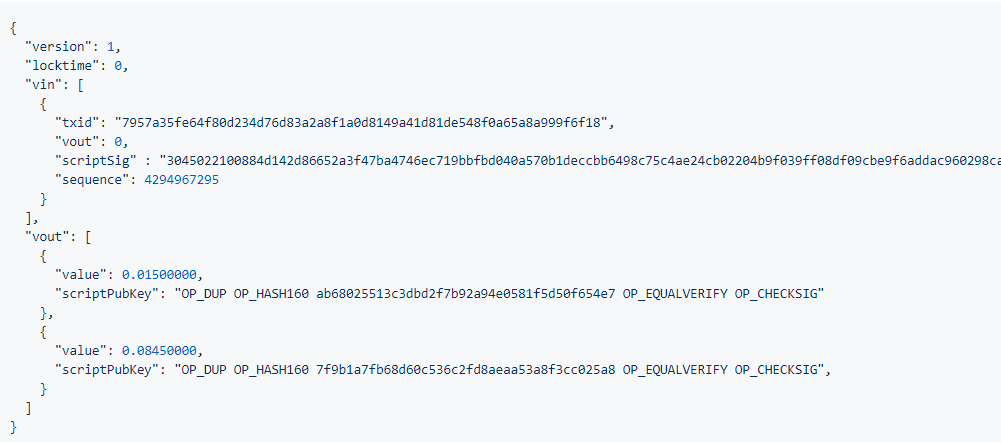
\includegraphics[width=\textwidth]{btc-tx.png}
    \end{center}
    \caption{A decoded Bitcoin transaction} \label{fig:btc-tx}
\end{figure}

A transaction is valid if the following conditions are fulfilled:

\begin{itemize}
    \item The total value of inputs is greater than or equal to the total value of outputs.
    \item For all $\varUTXO \opIn \varUTXO$ $\procVerfUTXO{\varUTXO} \opEqNoQ 1$ must hold.
    \item All input UTXOs have not been spent before.
    \item If a locktime $\varTime$ is given, the Bitcoin blockchain's current block needs to be higher or equal $\varTime$.
\end{itemize}

\begin{definition}[Bitcoin Transaction Scheme]
    We define a Bitcoin Transaction Scheme as a tuple of three DPT functions $(\procBuildTransactionId,
    \procSignTransactionId, \procVerfTransactionId)$.
    \begin{itemize}
        \item $\varBtcTx \opFunResult \procBuildTransaction{\varBtcInputs}{\varBtcOutpus}{\varVersion}{\varTime}$: The transaction building algorithm is a DPT function that takes as input a set of unspent transaction outputs $\varBtcInputs$, a collection of newly created transaction outputs $\varBtcOutpus$ a version number $\varVersion$ and an optional locking time $\varTime$.
        The algorithm will output an unsigned transaction $\varBtcTx$.
        \item $\funStar{\varBtcTx} \opFunResult \procSignTransaction{\varBtcTx}{\funArray{\varScriptSig}}$: The transaction
        signing algorithm is a DPT function that takes as input an unsigned Bitcoin transaction $\varBtcTx$ and an array
        of unlocking scripts $\funArray{\varScriptSig}$ for all transaction inputs.
        The algorithm outputs a signed Bitcoin transaction, which the sender can now broadcast to the network.
        \item $\{ 1,0 \} \opFunResult \procVerfTransaction{\varBtcTx}$: The verification algorithm is a DPT function taking as input a transaction $\varBtcTx$ outputting 1 on a successful verification or 0 otherwise.
        The function will check the well-balancedness of the transaction, verify the unlocking scripts, locktime and scan through the blockchain if all inputs are indeed unspent.
        Note that any public verifier with access to the blockchain ledger and $\varBtcTx$ is able to perform the verification.
    \end{itemize}
\end{definition}

We now outline two common structures of Bitcoin outputs the P2PK/P2PKH and the P2SH outputs.

\subsubsection{P2PK, P2PKH\label{sec:pre:bitcoin:p2pk}}

P2PK stands for Pay-to-Public-Key, and P2PKH for Pay-to-Public-Key-Hash.
In this type of output $\varScriptPubKey$ will be constructed such that its value unlocks if a correct signature is provided in $\varScriptSig$ for a corresponding public key $\varPubKey$.
P2PKH is an update to this script in which the $\varScriptPubKey$ contains a hashed version of the public key $\varPubKey$ instead of the public key itself.
To spend a P2PKH output, one has to provide the unhashed public key in addition to a valid signature.
This type of output is the most commonly used output in the Bitcoin blockchain to transfer value from one participant to another.
Delgado et al. found in their paper Analysis of the Bitcoin UTXO set from 2017 that more than 80\% of the UTXO set consisted of P2PKH transactions, whereas about 17\% were P2SH and 0.12\% P2PK outputs~\cite{delgado2018analysis}.
P2PKH outputs can be encoded into a Bitcoin address using base58 encoding.
These addresses can be handed out to request a payment from somebody.

\subsubsection{P2SH} \label{sec:pre:bitcoin:p2sh}

If more advanced spending conditions, such as multi-signature, are required, P2SH (Pay-to-script-hash), introduced in 2012, is a way to implement those in a space-efficient and straightforward matter.
Here the locking condition $\varScriptPubKey$ does not contain a script but instead the hash of a script.
Upon spending, the spender has to provide the original script and the unlocking requirements for the script itself.
Upon verification, the provided script's hash will be computed and compared with the value given in the locking condition.
If those match, the actual script will be executed.
The advantage of using this approach over just handcrafting a custom locking script is that the locking scripts are relatively short, making the transactions smaller, reducing fees, or shifting them from the sender to the output owner.
Additionally, this type of output can be encoded again into a Bitcoin address similar to a P2PKH output, making it easy to request a payment.